\section{Attacking Property-preserving Encryption}


Since we developed the code for this assignment using Java, the project code is written in the .txt file separated by file name. The code is also accessible on \href{https://github.com/lallo-unitn/secure_cloud_assignment2/tree/main/cryptoDB/cryptodbProject/src/main/java/nl/ut/eemcs/cloudsec}{GitHub}.

\subsection{Number of unique first names in the database}

In the database, there are 100 unique first names stored. This number was determined by taking into consideration that the names in the database were encrypted using deterministic encryption. As a consequence, the number of unique encrypted first names is equivalent to the number of first names in the database.

\begin{lstlisting}[language = Java, caption=Java Code to Count Unique First Names, firstnumber = last , escapeinside={(*@}{@*)}]
    public int getFirstNameCount() {
        String query = "SELECT COUNT(DISTINCT enc_firstname) FROM enc_students";
    
        try (Connection conn = DriverManager.getConnection(url);
             PreparedStatement pstmt = conn.prepareStatement(query);
             ResultSet rs = pstmt.executeQuery()) {
    
            if (rs.next()) {
                return rs.getInt(1);
            }
    
        } catch (SQLException e) {
            System.out.println("Error: " + e.getMessage());
        }
        return 0;
    }
\end{lstlisting}

\newpage

\subsection{Distribution of last names}

To plot the distribution of the encrypted last names we determined the number of occurrences of each last name present in the database.

Following is the code to compute the last name frequency.

\begin{lstlisting}[language = Java, caption = Distribution of last names, firstnumber = last , escapeinside={(*@}{@*)}]

    public HashMap<String, Integer> getLastnameFrequenciesOrdered() {
        String query = "SELECT enc_lastname FROM enc_students";

        try (Connection conn = DriverManager.getConnection(url);
             PreparedStatement pstmt = conn.prepareStatement(query);
             ResultSet rs = pstmt.executeQuery()) {

            HashMap<String, Integer> lastnameFrequencies = new HashMap<>();
            while (rs.next()) {
                String lastname = rs.getString("enc_lastname");
                if (lastnameFrequencies.containsKey(lastname)) {
                    lastnameFrequencies.put(lastname, lastnameFrequencies.get(lastname) + 1);
                } else {
                    lastnameFrequencies.put(lastname, 1);
                }
            }
            
            return orderHashMapByValue(lastnameFrequencies);

        } catch (SQLException e) {
            System.out.println("Error: " + e.getMessage());
        }
        return null;
    }
\end{lstlisting}

Following, the graph with lastnames in chipertext.

\begin{figure}[H]
    \centering
    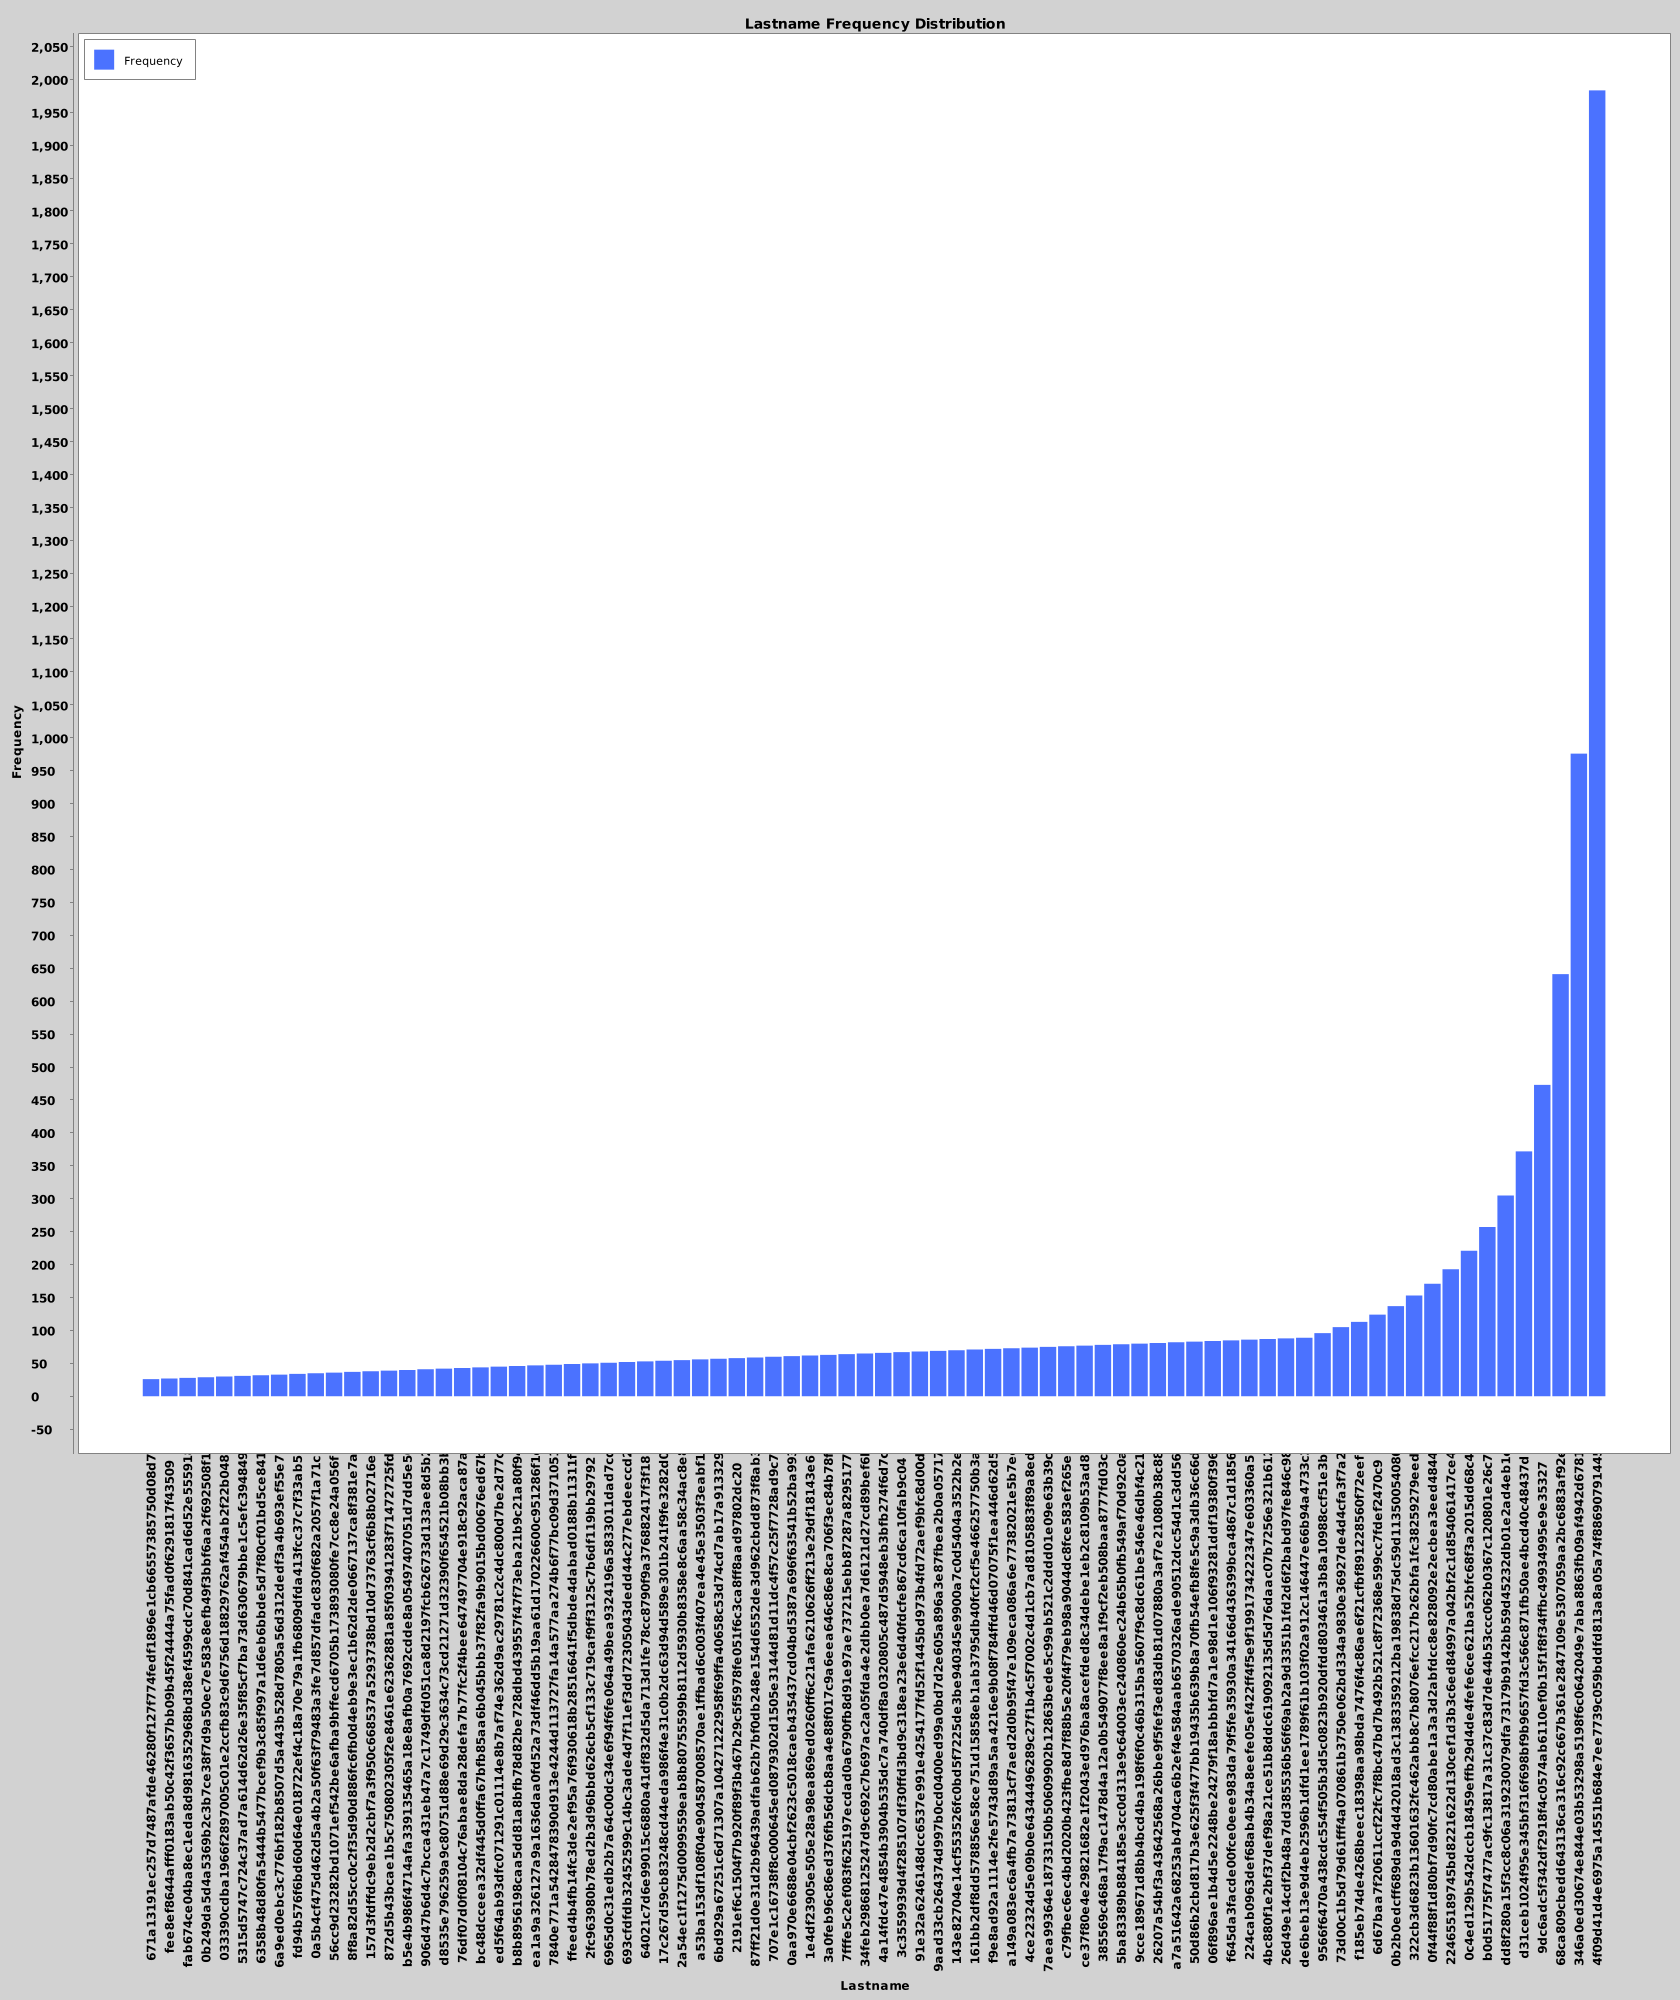
\includegraphics[width=\textwidth]{03-ex2/Lastname_Frequency_Distribution.png}
    \caption{Distribution of encrypted last names.}
    \label{fig:Distribution-of-last-names}
\end{figure}

The graph shows the distribution of the encrypted last names names. The distribution is clearly non-uniform, and an attacker can use background information (like the files given for this assignment) to infer by crafting a lookup table for mapping encrypted values to plaintext values.

Following, the same graph with names in plaintext.

\begin{figure}[H]
    \centering
    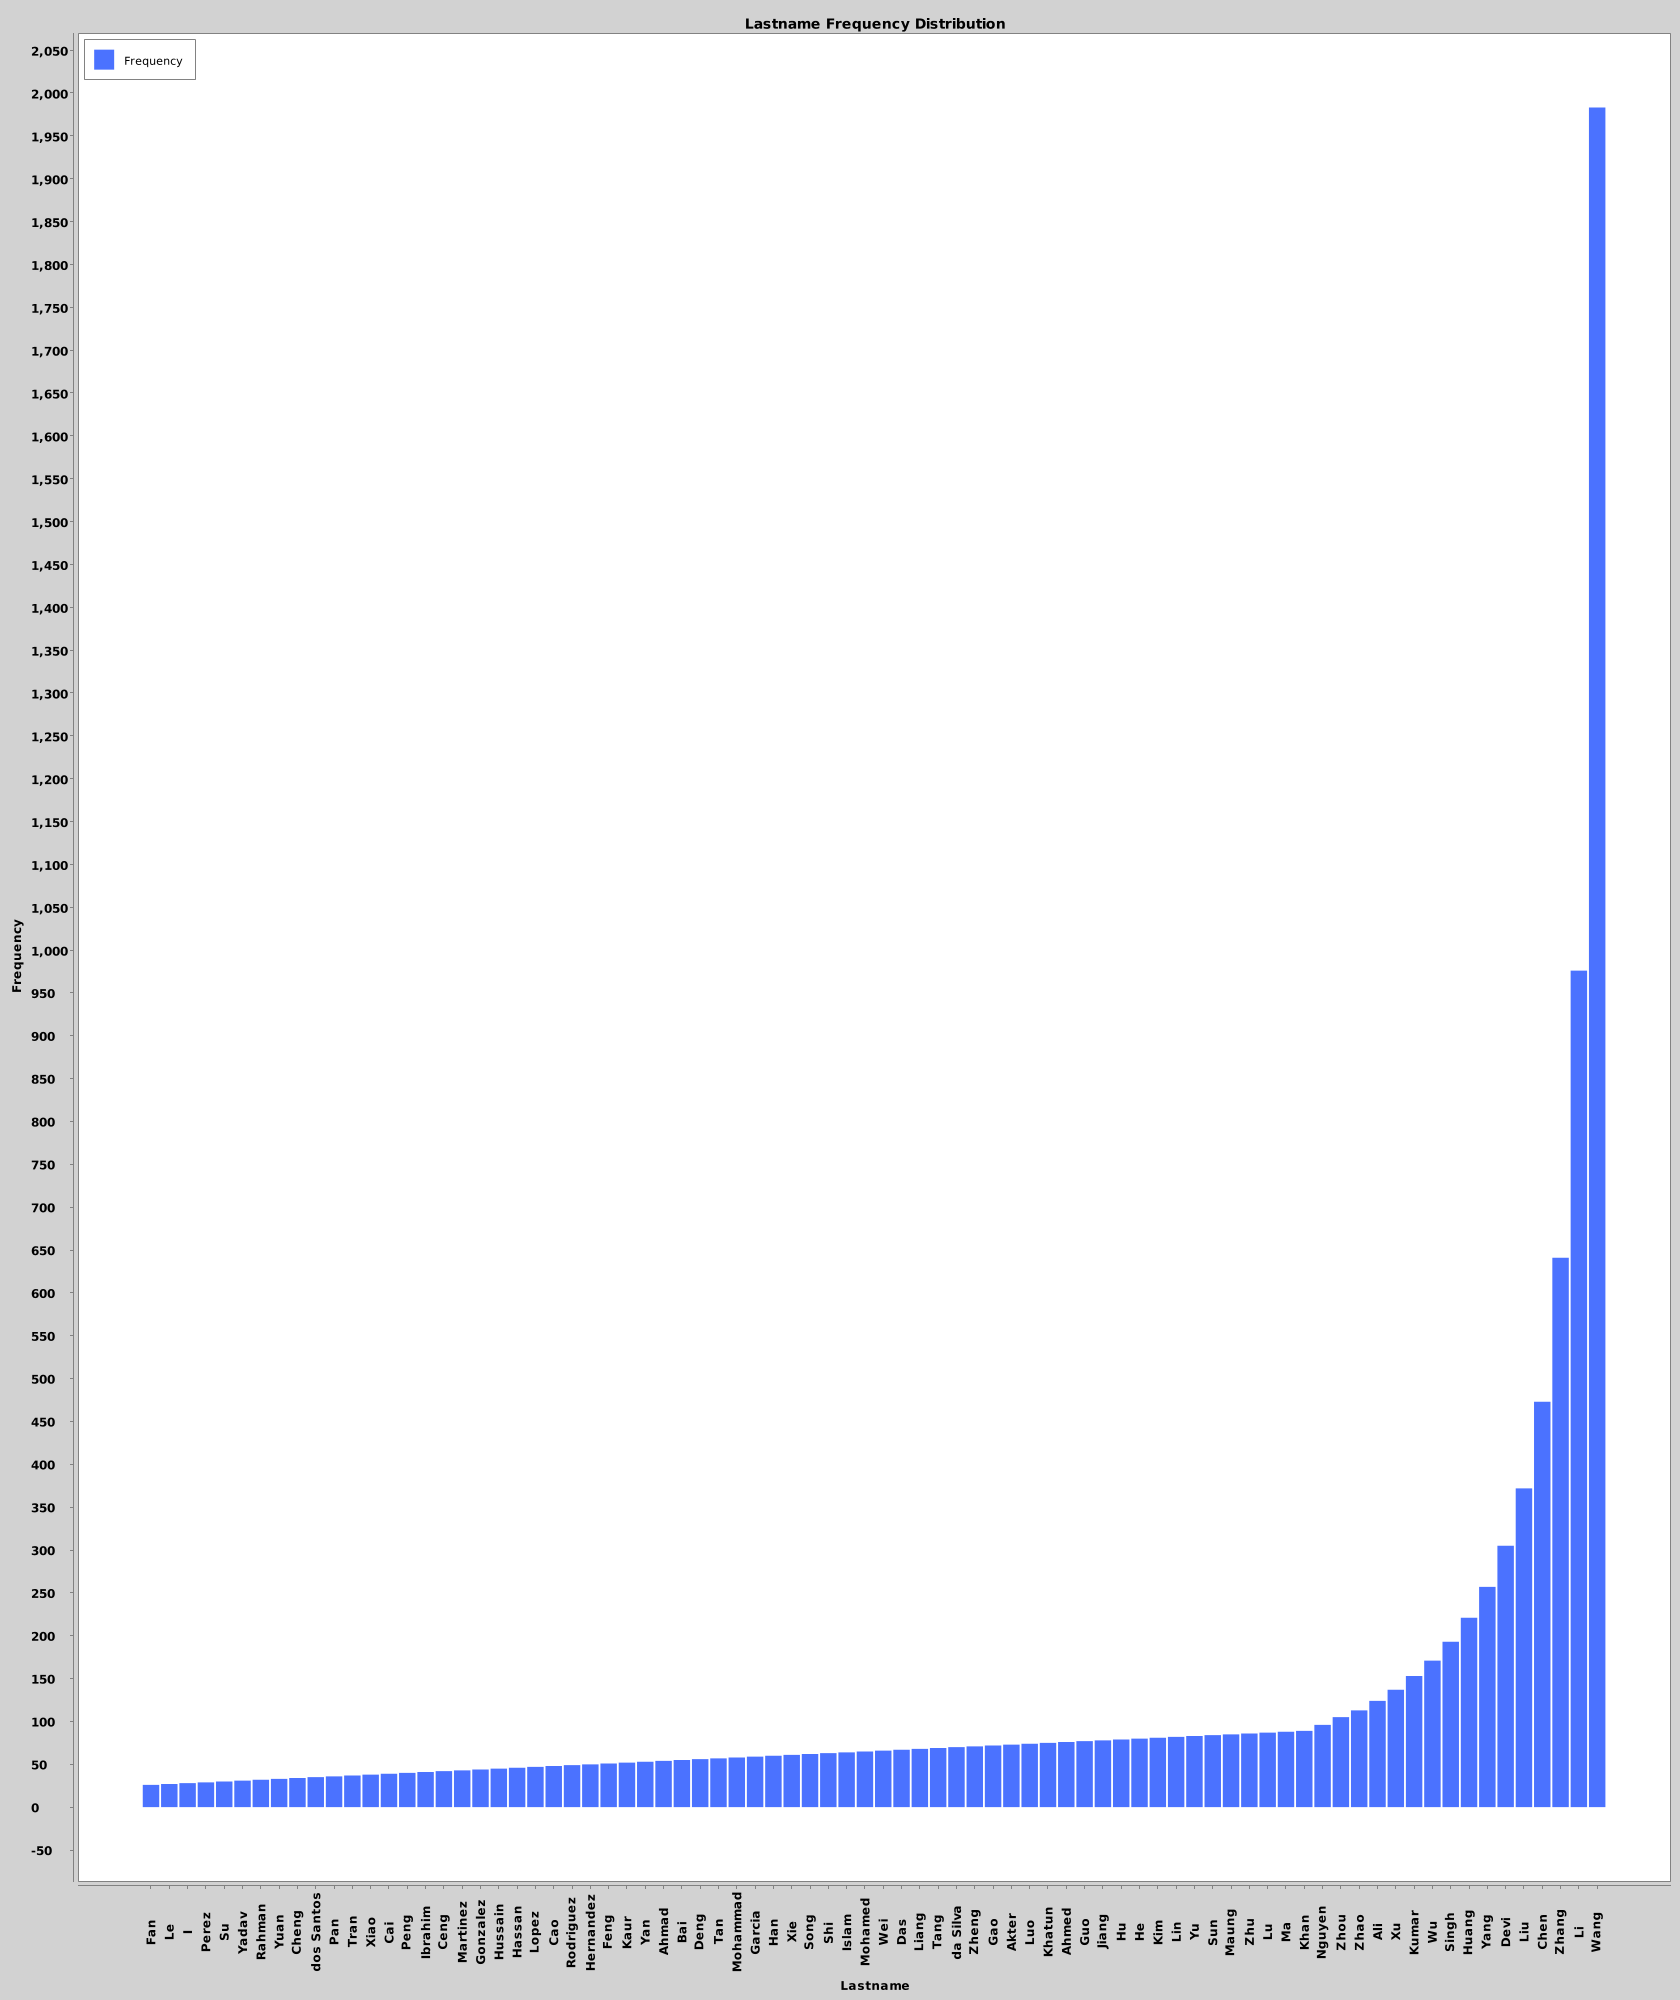
\includegraphics[width=\textwidth]{03-ex2/Lastname_Frequency_Distribution_Plain.png}
    \caption{Distribution of the last names in plaintext.}
    \label{fig:Distribution-of-last-names-plain}
\end{figure}

As it can be seen, the last name Wang (which is the most popular last name) is mapped to the ciphertext \\ \texttt{4f09d41d4e6975a14551b684e7ee7739c059bddfd813a8a05a74f88690791445}.

\newpage
\subsection{Full names of all students who scored 99 points}

There are 100 unique values stored in the database for grades. We also know that the grades can range from 1 to 100. This means that the data set for the grades is a dense dataset since the complete plaintext space is encrypted. Since the grades are encrypted in an order-preserving manner, the lower numeric value of an encrypted grade corresponds to a lower plaintext value. Based on this information, we sorted the ciphertexts decreasingly, this is how we were able to recover the ciphertext value corresponding to 99.

Following that, we queried all the records where the value of the grade was the previously determined one and we got the students who scored 99 points. The encrypted names could be mapped to the plaintext ones based on the given txt files (again, by leveraging the use of deterministic encryption).

In total there were 149 records with the grade of 99, belonging to 129 students, whose names' are the following: Abdul Yan, Ahmad Cai, Ahmed He, Ahmed Huang, Ahmed Tran, Ali Chen, Ali Martinez, Ana Singh, Ana Zheng, Andrea Mohammad, Andrey Huang, Anna Yang, Antonio Feng, Antonio I, Antonio Xu, Bin Hernandez, Carlos Su, Carlos Yang, Carlos Yu, Carmen Cao, Charles Peng, Daniel Han, David Devi, David Lu, David Zhang, Elena Liu, Elena Wang, Elizabeth Deng, Fatima Khatun, Fatima Wang, Francisco Gao, Francisco Gonzalez, George Kumar, Hong Singh, Hui Cao, Hui Kaur, Hui Liu, Hui Wang, Ibrahim Hassan, Ibrahim Khatun, James Chen, James Zheng, Jean Gao, Joao Ceng, John Li, John Luo, John Singh, John Sun, Jorge Akter, Jorge Chen, Jorge dos Santos, Jose Chen, Jose Li, Jose Tan, Jose Yu, Jose Zhang, Joseph Zhang, Juan Le, Juan Yang, Laura Pan, Lei Hu, Lei Jiang, Lei Wu, Li Li, Li Luo, Ling Xiao, Luis Tan, Manuel Ahmed, Manuel Shi, Maria Li, Maria Wang, Maria Zhang, Marie Gonzalez, Marie Guo, Mario Lin, Mario Yang, Mark Bai, Mark Tan, Martha Tran, Martin Pan, Mary Li, Michael Zhang, Min He, Ming Ahmed, Ming Han, Ming Tang, Mohamed Li, Mohamed Liu, Mohamed Wu, Mohamed Zhang, Mohammed Chen, Mohammed Li, Mohammed Wang, Mohammed Zhang, Muhammad Chen, Muhammad Hu, Muhammad Luo, Nushi Chen, Nushi Li, Nushi Liu, Nushi Wang, Nushi Zhang, Olga Maung, Patrick Zhu, Paul Shi, Peter Luo, Ram Gonzalez, Ram Peng, Richard Liu, Richard Ma, Robert Wu, Rosa Devi, Rosa Wang, Samuel Rodriguez, Samuel Zheng, Sandra Ahmed, Sergey Deng, Sergey Hernandez, Sergey Luo, Siti Khan, Siti Pan, Sri Wu, Wei Chen, Xin Yang, Ying Khan, Ying Wang, Yong Zhu, Yu Deng, Yu Zhu.

\begin{lstlisting}[language = Java, caption = Querying for the students who got 99, firstnumber = last , escapeinside={(*@}{@*)}]
public String getSecondUniqueHighestValue() {
        String query = "SELECT enc_grade FROM ("
                + "    SELECT DISTINCT enc_grade"
                + "    FROM enc_students"
                + "    ORDER BY enc_grade DESC"
                + ") as eseg LIMIT 1 OFFSET 1;";

        try (Connection conn = DriverManager.getConnection(url);
             PreparedStatement pstmt = conn.prepareStatement(query)) {

            // Execute the query
            ResultSet rs = pstmt.executeQuery();

            // Process the result
            if (rs.next()) {
                return rs.getString("enc_grade");
            }
        } catch (SQLException e) {
            System.out.println(e.getMessage());
        }
        return null;
    }

    public List<Student> getSecondToTopStudents() {
        String secondValue = getSecondUniqueHighestValue();
        String query = "SELECT enc_firstname, enc_lastname FROM enc_students WHERE enc_grade = ?";
        List<Student> resultList = new ArrayList<>();

        try (Connection conn = DriverManager.getConnection(url);
             PreparedStatement pstmt = conn.prepareStatement(query)) {

            pstmt.setString(1, secondValue);
            ResultSet rs = pstmt.executeQuery();

            ResultSetMetaData metaData = rs.getMetaData();
            int columnCount = metaData.getColumnCount();

            while (rs.next()) {
                Student student = null;
                for (int i = 1; i <= columnCount; i++) {
                    student = new Student(
                            rs.getString("enc_firstname"),
                            secondValue,
                            rs.getString("enc_lastname")
                    );
                }
                resultList.add(student);
            }

        } catch (SQLException e) {
            System.out.println("Error: " + e.getMessage());
        }

        return resultList;
    }
\end{lstlisting}
\newpage
\subsection{Implementing $(\alpha, t)$-secure index as mitigation}

The main idea behind the $(\alpha,t)$-secure index is to protect against inference attacks by adding noise to the data in a structured way via clustering the result sets into different partitions. The $\alpha$ parameter specifies the minimum number of keywords that must share a similar access pattern. A higher $\alpha$ means more keywords will be grouped together, increasing privacy but possibly introducing more noise. The $t$ parameter indicates the maximum allowable Hamming distance (i.e., the number of differing bits) between the access patterns of keywords within the same group. A smaller $t$ ensures more similarity between access patterns, improving privacy but potentially leading to more false positives during search results.

We implemented a $(4,0)$-secure index by a lookup function, which when searched for by their last names, returns results clusters of 4 keywords. This leads to confusing results when an adversary tries to map the distribution of names similarly to how it was described previously, but it also introduces multiple false positives returned by also returning results for the other 3 keywords, with which the client executing the query has to parse to identify.

Following, is the graph of last name frequencies after implementing a $(4, 0)$-secure index search. As it can be seen, the previous easily mappable distribution is gone, instead, clusters of 4 appeared.

\begin{figure}[H]
    \centering
    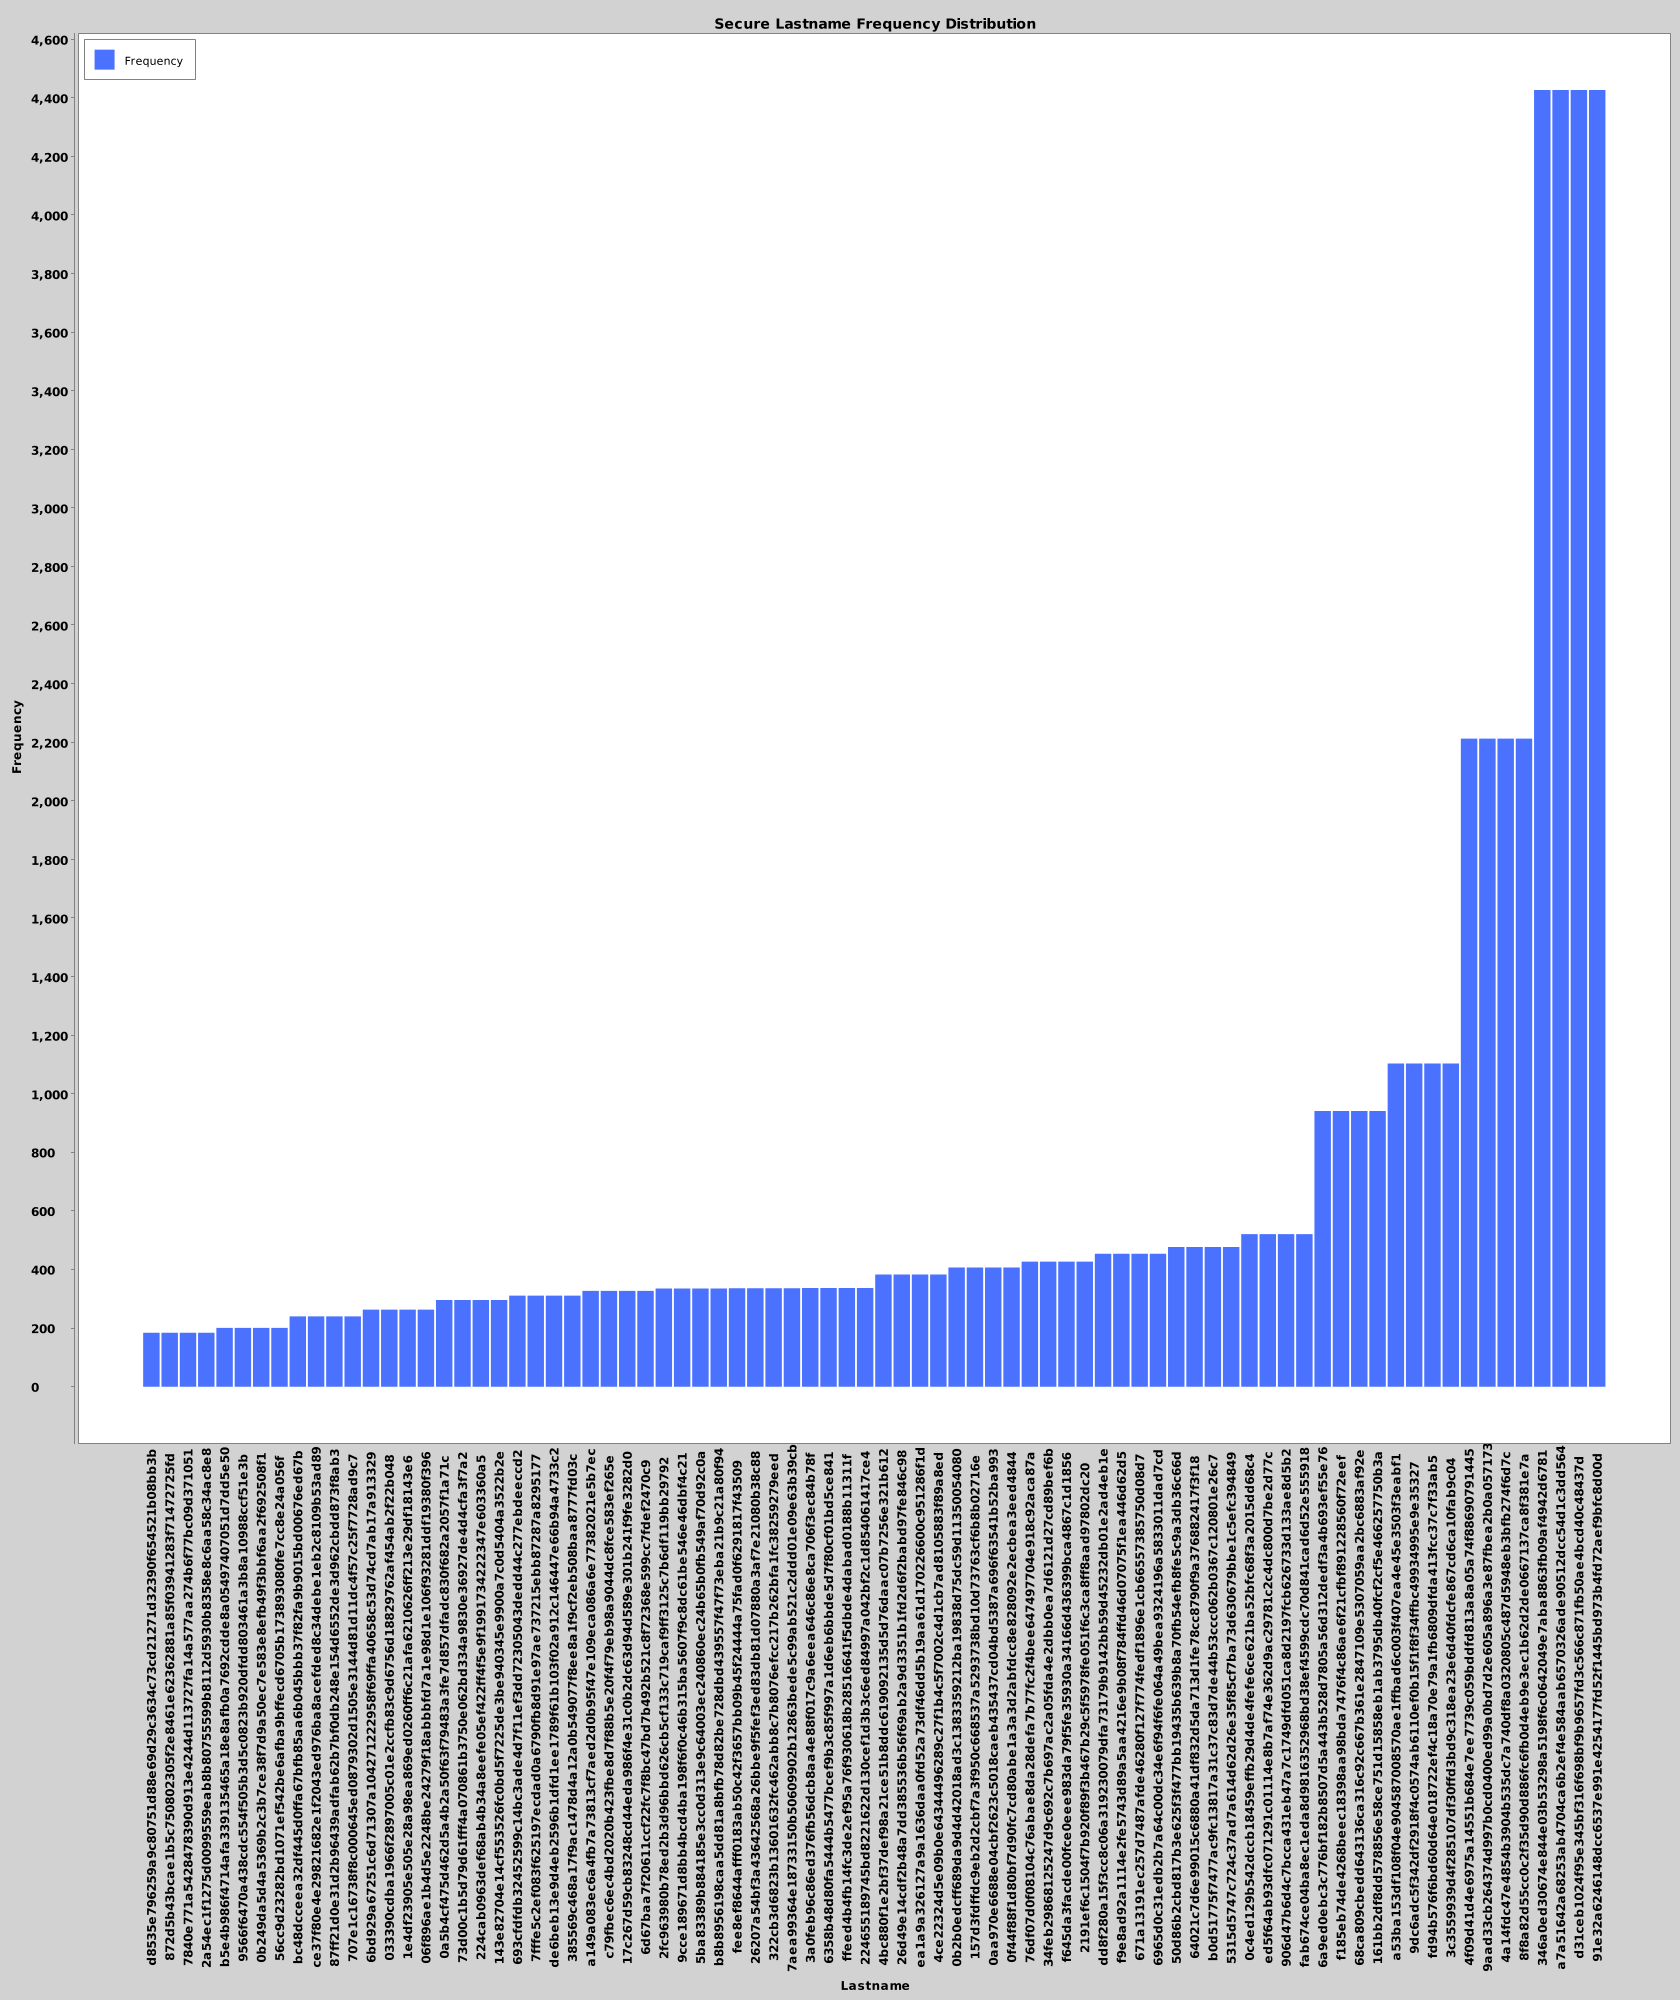
\includegraphics[width=\textwidth]{03-ex2/Secure_Lastname_Frequency_Distribution.png}
    \caption{Distribution of encrypted last names with (4,0)-secure index.}
    \label{fig:Distribution-of-last-names-sec}
\end{figure}

When looking at the plaintext equivalents of the last names from the previous graph, it can also be observed, that only the distribution changed, but so did the few most frequent last names too.

\begin{figure}[H]
    \centering
    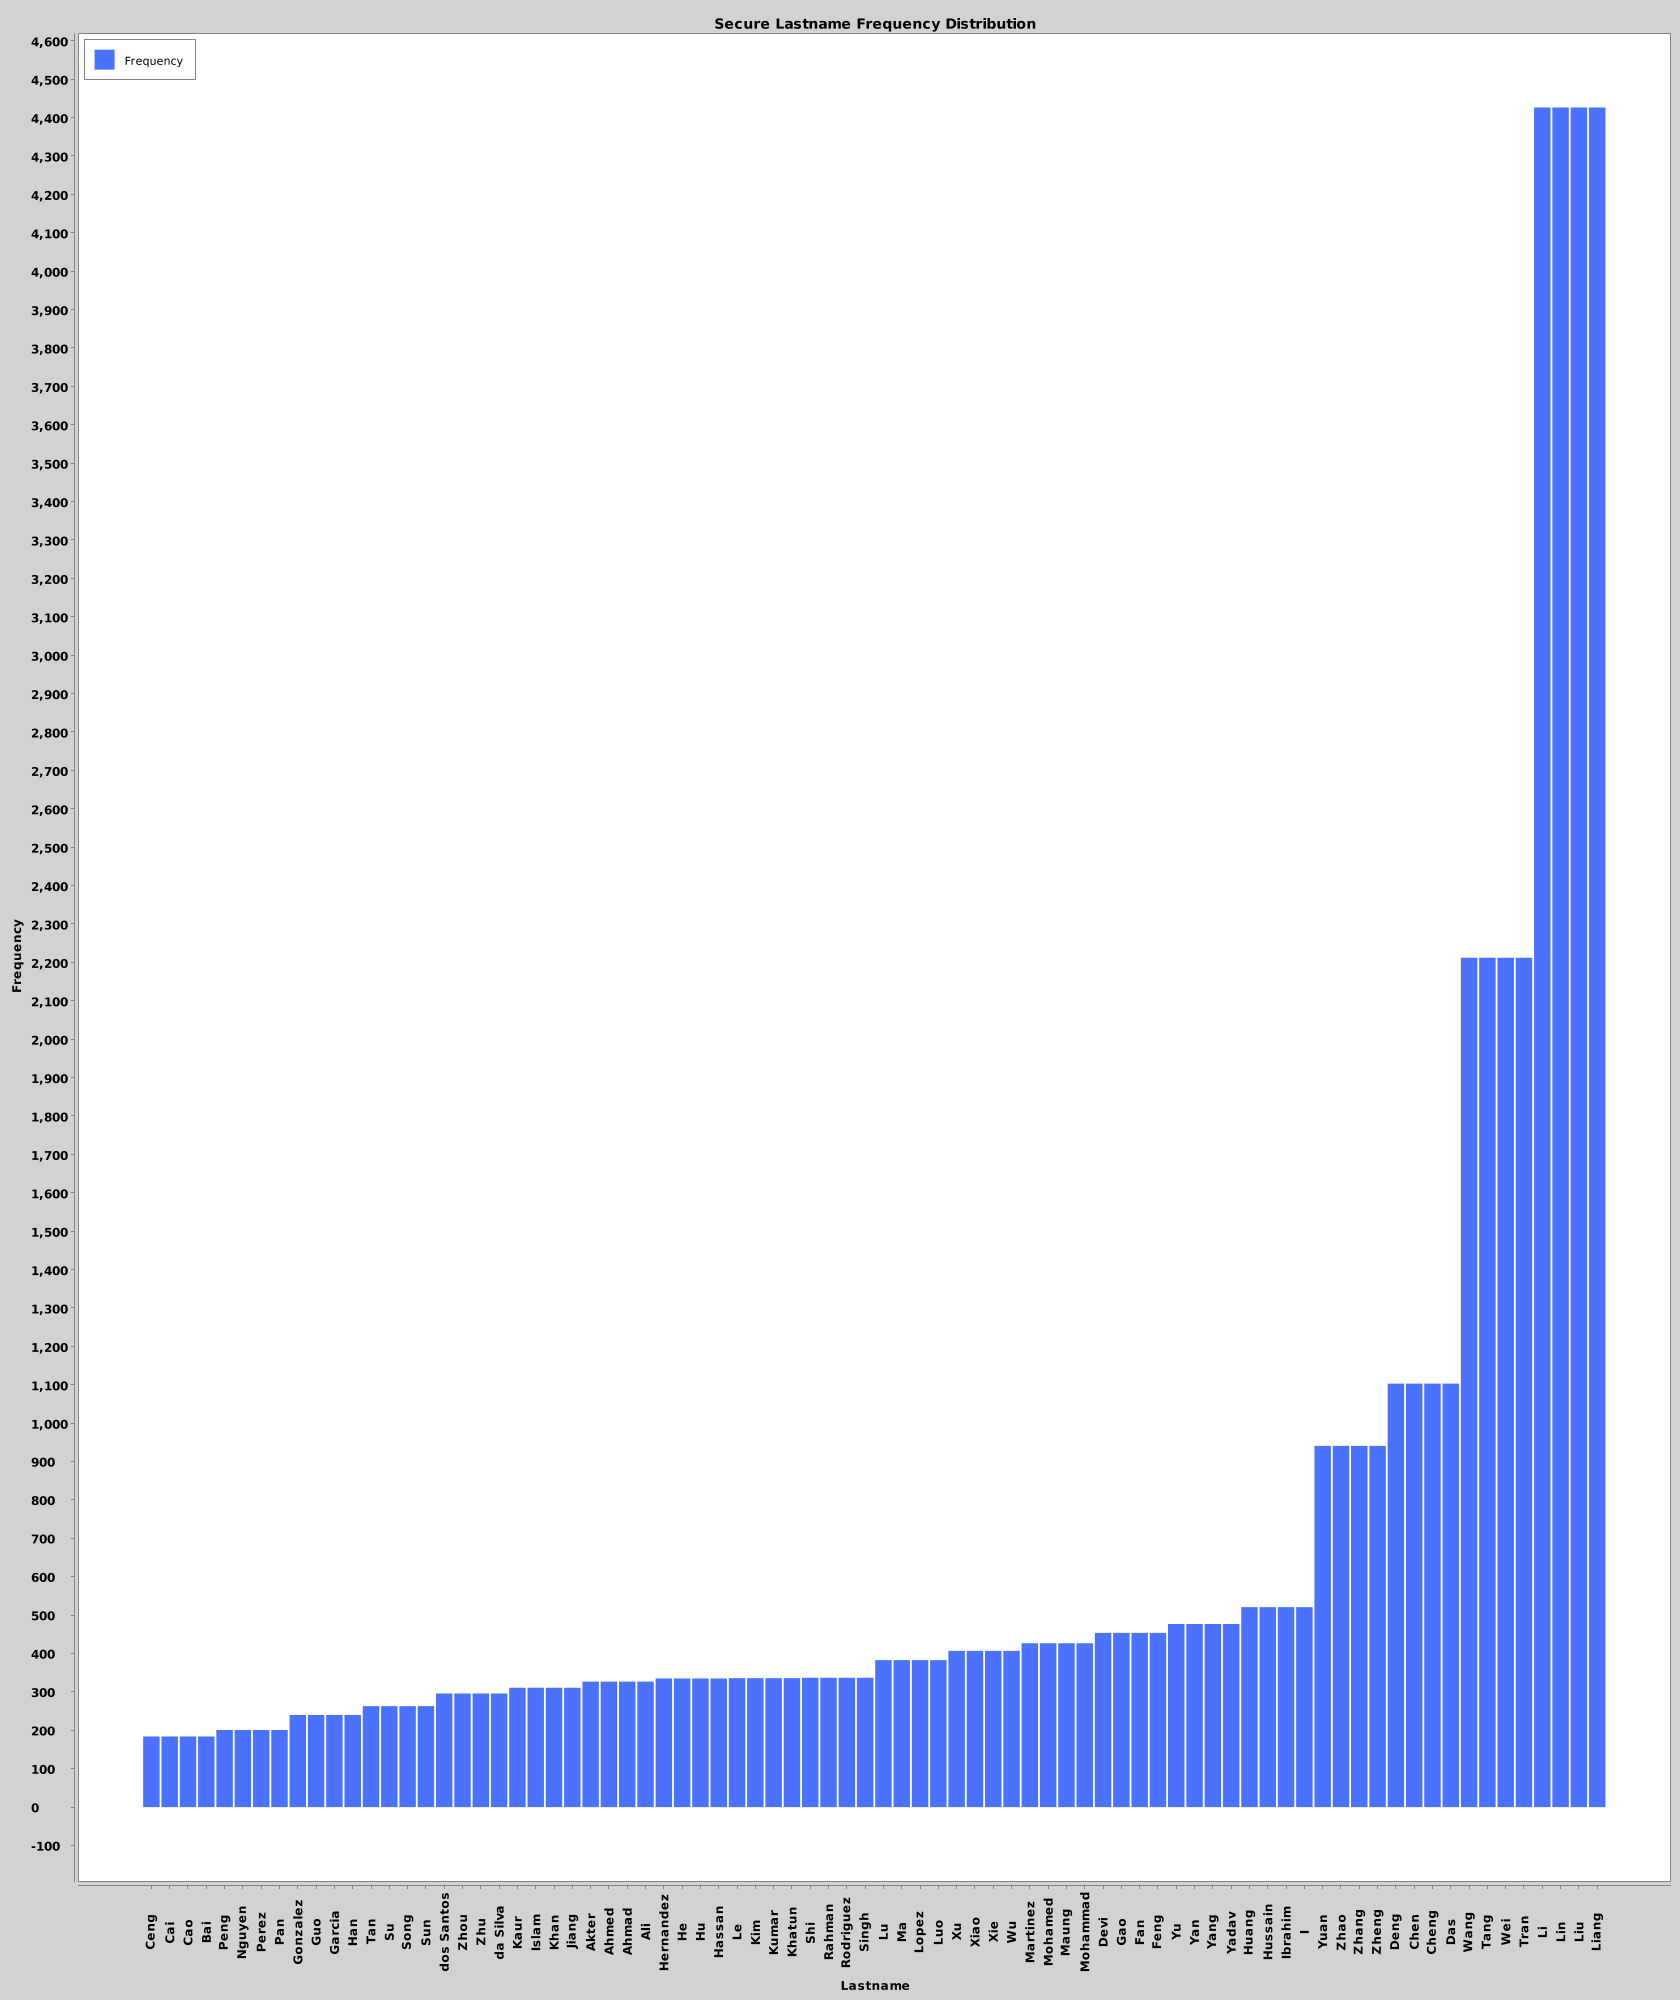
\includegraphics[width=\textwidth]{03-ex2/Secure_Lastname_Frequency_Distribution_Plain.png}
    \caption{Distribution of the last names in plaintext with (4,0)-secure index.}
    \label{fig:Distribution-of-last-names-plain-sec}
\end{figure}


Following, the code 

\begin{lstlisting}[language = Java, caption = secure index as mitigation, firstnumber = last , escapeinside={(*@}{@*)}]

    public List<Student> getSecStudentsFromSurname(String surname, int alpha) {
        List<Student> students = new java.util.ArrayList<>();
        int i = surnameList.indexOf(surname);

        //compute cluster boundaries
        int clusterUpperBound = i;
        for (int j = i; (j % alpha != 0 || j==i) && (j<rows); j++) {
            clusterUpperBound = j;
        }
        int clusterLowerBound = i;
        for (int j = i; (j % alpha != 0) && j>0 ; j--) {
            clusterLowerBound = j-1;
        }

        //return students in alpha-size cluster
        if(i != -1) {
            for (int j = i; j <= clusterUpperBound && (j<rows); j++) {
                for (int k = 0; k < cols; k++) {
                    if (matrix[j][k]) {
                        students.add(studentList.get(k));
                    }
                }
            }
            i--;
            for (int j = i; j >= clusterLowerBound; j--) {
                for (int k = 0; k < cols; k++) {
                    if (matrix[j][k]) {
                        students.add(studentList.get(k));
                    }
                }
            }
        }

        return students;
    }
\end{lstlisting}